\section[\LaTeX 极速入门]{\LaTeX 极速入门\protect\footnotemark}
\footnotetext{该部分的内容为科普向，如已对 Git，GitHub，LaTeX 均已熟悉，可略过该章}
\label{sec:use}

\subsection{Git 与 GitHub}
\label{sec:github}

Git 是一种版本控制工具，用于记录文件在不同时间的修改情况。
我们可以用它来保存论文和分析代码的修改历史，比较不同版本之间的差异，并在需要时找回此前的内容。
更直观地讲，它是一个手动触发的时光机。
例如，我们在调整样本范围并重新估计模型后，可以将相关修改提交，后续如果发现问题，可以找回之前版本的代码，而不需要用诸如 \texttt{final-261111-real-final-v10-打死都不改了版-再改就吐血了.docx} 这样的命名存档。

我们也可以用数学语言进行介绍，设第 $t$ 次提交所记录的文件状态为 $S_t$，从该版本到下一版本的改动为 $\Delta_t$。在沿同一条分支持续修改的情况下，下一版本可以表示为
\[
    S_{t+1} = \mathrm{Apply}(S_t, \Delta_t).
\]
其中，$\mathrm{Apply}$ 表示将改动应用到文件上。Git 的每次提交可表示为
\[
    C_t = (S_t, P_t, M_t).
\]
$S_t$ 是提交时的文件快照，记录的是版本控制中已跟踪文件的状态，以及本次提交中新增或修改的文件；尚未加入提交的修改和被忽略的文件不会自动保存。
$P_t$ 是该次提交直接接续的提交集合，$M_t$ 包含作者、时间和修改说明。

若每次提交都接续上一次提交，版本历史形成一条链
\[
    C_0 \longrightarrow C_1 \longrightarrow C_2.
\]
若两位合作者从同一版本 $C_0$ 出发，分别修改正文和分析代码，再将两人的修改合并，并生成一个合并提交，版本历史可以表示为
\[
    C_0 \longrightarrow
    \left\{
    \begin{array}{l}
        C_1^{(A)} \\
        C_1^{(B)}
    \end{array}
    \right\}
    \longrightarrow C_2^{(\mathrm{merge})}.
\]
其中，合并提交 $C_2^{(\mathrm{merge})}$ 同时接续 $C_1^{(A)}$ 和 $C_1^{(B)}$。由此，Git 的版本历史可以表示为有向无环图，其中每个节点对应一次提交，箭头从较早的提交指向接续它的提交。

GitHub 是一个基于 Git 的在线托管与协作平台。
研究者可以将论文的 \LaTeX 源文件、参考文献和分析代码放在同一个仓库中，与合作者共享。
合作者可以在线查看每次提交改动了哪些文件，也可以提交拟议的修改，由其他成员审阅和讨论后再将其纳入共同维护的稿件。

研究者可以使用 GitHub 上的模板仓库创建自己的论文项目。
这里以图~\ref{fig:github-paper-template} 所示的 AIdea-Labs 内部模板为例，点击页面右上方的 \textbf{Use this template}，再选择 \textbf{Create a new repository}，即可在自己的账户下新建一个包含该模板项目文件的新仓库。
新仓库从一条初始提交开始，与原模板仓库不共享提交历史，此后可以独立记录论文的修改过程。
如果你希望向模板仓库贡献修改，可以通过 \textbf{Fork} 按钮创建一个与原仓库关联的副本，在自己的副本中修改后，向原项目提交 \textbf{Pull Request}（简称 PR），请求维护者检查并合并这些修改。
由于基于模板创建的仓库与原仓库没有共同的提交历史，通常不能直接向原模板仓库提交 PR。
因此，使用模板写自己的论文可以选择 \textbf{Use this template}，向模板项目贡献修改则可以选择 \textbf{Fork}。

\begin{figure}[htbp]
    \centering
    \setlength{\unitlength}{\linewidth}
    \begin{picture}(1,0.501)
        \put(0,0){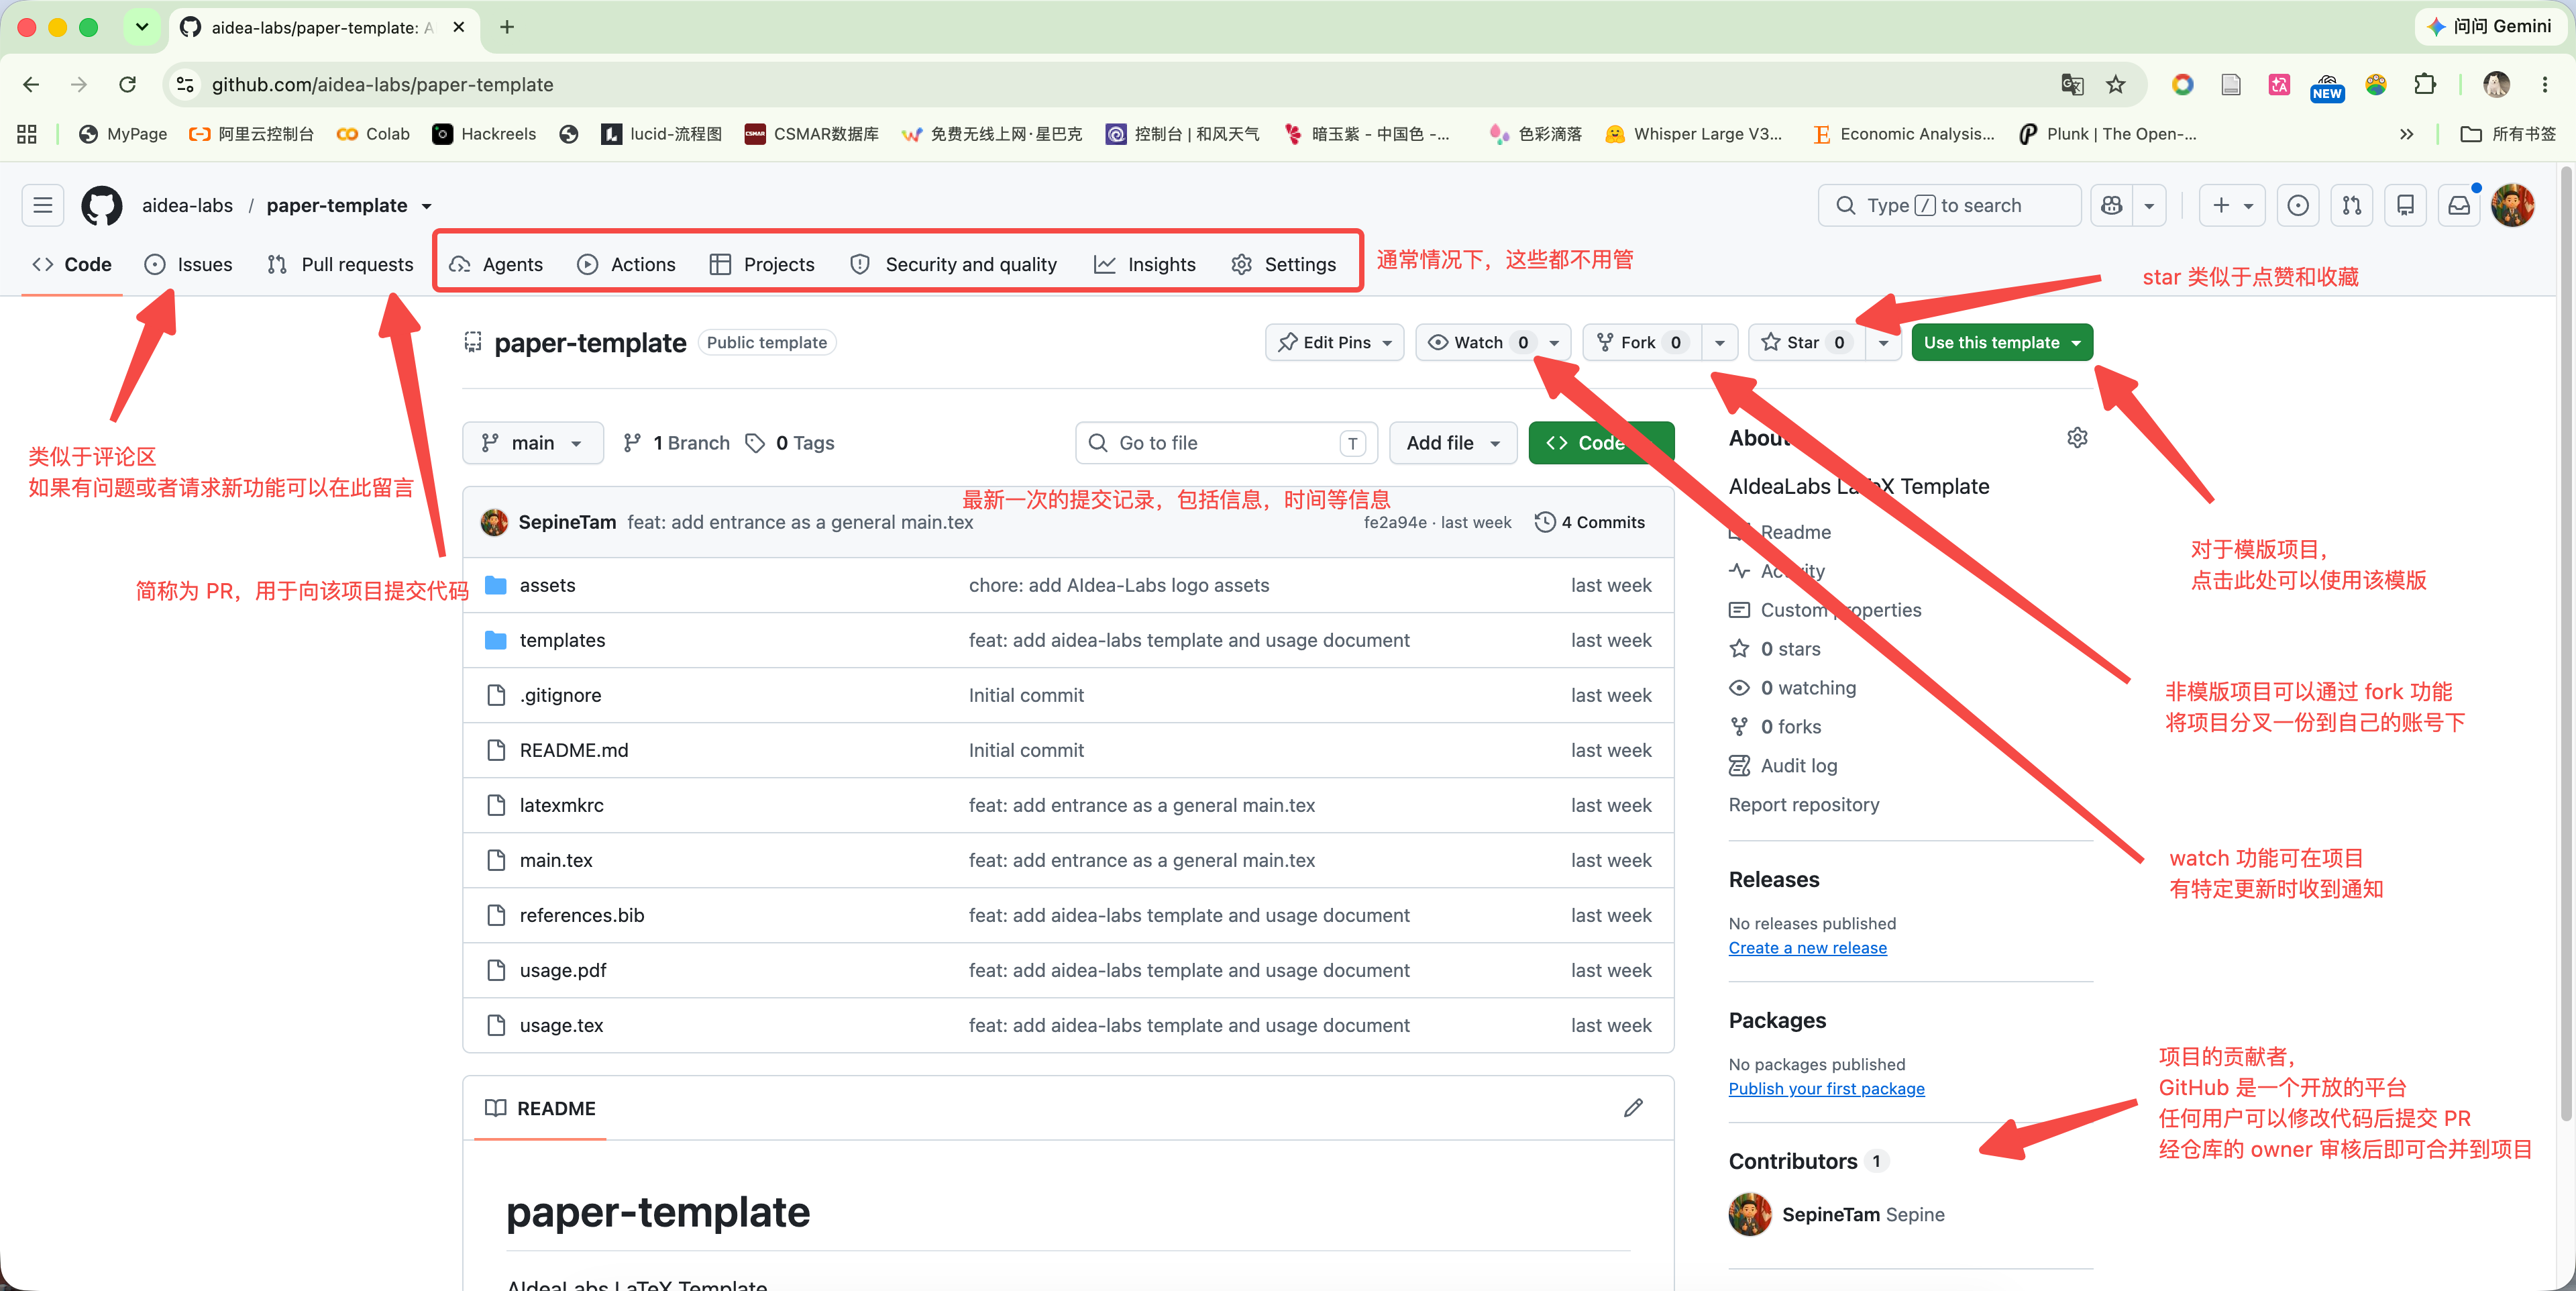
\includegraphics[width=\linewidth]{figs/github-paper-template.png}}
        \put(0.835,0.215){\colorbox{white}{\parbox[b][0.024\linewidth][c]{0.164\linewidth}{\color{red}\fontsize{3.6}{4.5}\selectfont 希望向原项目贡献修改时，\\可以通过 Fork 创建副本。}}}
    \end{picture}
    \caption{以 AIdea-Labs 论文模板为例的 GitHub 仓库界面}
    \label{fig:github-paper-template}
    \par\smallskip
    {\footnotesize\raggedright
    \textbf{注：}该图片截图并批注于 2026 年 11 月 11 日。
    图中为 GitHub 上 \texttt{aidea-labs/paper-template} 的仓库首页。
    红色箭头和文字为作者所加，标出了创建模板副本、分叉、查看提交记录、反馈问题和提交修改请求等位置。
    图中展示的是 AIdea-Labs 的另一个模板项目；本文项目可以\href{https://github.com/aidea-labs/econ-sbm-template}{\underline{点击这里}}查看。
    \par}
\end{figure}

仓库首页的 \textbf{Code} 页面列出项目文件，并在文件列表上方显示最近一次提交及其时间。
点击提交记录，可以查看该版本具体修改了哪些文件。
使用模板时，遇到编译问题或希望增加某项功能，可以在 \textbf{Issues} 中提出；如果已经修改了模板，也可以通过 \textbf{Pull requests} 提交改动，供维护者查看和讨论。
\textbf{Star} 可用于收藏项目，\textbf{Watch} 则用于订阅所关心的更新。

\subsection{使用模板撰写论文}
\label{sec:how}

研究者可以先获取模板，再填写论文内容、选择期刊格式并编译为 PDF。
如果已经有 GitHub 账号，可以\href{https://github.com/new?template_name=paper-template&template_owner=aidea-labs}{\underline{点击这里}}使用 AIdea-Labs 的通用论文模板，在自己的账号下创建一个新仓库。
如果还没有 GitHub 账号，我们建议先创建一个账号，以便创建自己的论文仓库，并在后续与合作者共享和管理论文。
如果不想创建账号，也可以使用 Git 直接克隆公开仓库，在本地获取模板并开始写作。

获取模板后，可以先看看项目的文件结构，而不必急着修改期刊格式。
在本文的示例中，\texttt{main.tex} 是论文的入口，包含论文标题、作者、摘要、关键词以及正文各部分的调用；\texttt{sections} 目录存放引言、相关工作等正文内容，\texttt{ref.bib} 存放参考文献，\texttt{figs} 目录存放图片，\texttt{templates} 目录则存放不同的文档类文件。
这样安排的好处是，研究者可以把注意力放在论文内容上，同时让各部分保持相对独立。

开始写作时，可以先在 \texttt{main.tex} 中填写论文的标题、作者、摘要和关键词，再根据自己的需要修改正文。
如果一篇论文包含引言、文献综述、研究设计和结论等部分，可以将它们分别放在 \texttt{sections} 目录的不同文件中，并通过 \verb|\input{...}| 在 \texttt{main.tex} 中按顺序调用。
正文中的章节层级则可以使用 \verb|\section|、\verb|\subsection| 和 \verb|\subsubsection| 表示，具体的标题样式由所选模板处理。

在论文中添加公式时，可以使用 \texttt{equation} 环境生成带编号的公式，并通过 \verb|\label| 为公式设置一个便于识别的名称。
例如，样本均值可以写为
\begin{equation}
    \bar{x}=\frac{1}{n}\sum_{i=1}^{n}x_i.
    \label{eq:sample-mean}
\end{equation}
在式~\eqref{eq:sample-mean} 中，$n$ 是样本量，$x_i$ 是第 $i$ 个观测值，$\bar{x}$ 是样本均值。
这里的引用使用 \verb|\eqref{eq:sample-mean}|，其中 \texttt{eq:sample-mean} 与公式中的标签一致，因此后续增删或调整公式时，无需手动修改正文中的编号。

图表的处理方式与公式类似：先在图或表的环境中添加标题和标签，再在正文中通过 \verb|\ref| 引用。
例如，本文在前文通过表~\ref{tab:word-latex} 对比 \LaTeX{} 和 Word，又通过图~\ref{fig:github-paper-template} 介绍 GitHub 仓库的界面。
正文中的编号由 \LaTeX{} 根据标签生成，即使图表的排列顺序发生变化，也可以在重新编译后更新对应的引用。
表格可以使用 \texttt{booktabs} 宏包提供的命令绘制三线表，图片则可以放在 \texttt{figs} 目录中，再使用 \verb|\includegraphics| 插入。

\begingroup
\sloppy
参考文献集中放在 \texttt{ref.bib} 中，每一条文献都有一个引用键。
例如，\texttt{james\_does\_2026} 对应 \textcite{james_does_2026}，在正文中写入 \verb|\textcite{james_does_2026}| 就可以引用该文献。
如果需要将作者和年份一起放在括号中，也可以使用 \verb|\parencite{james_does_2026}|，得到如 \parencite{james_does_2026} 所示的效果。
文末参考文献由 \verb|\printbibliography| 生成，文内引文和文末条目的具体形式则由当前模板的参考文献样式决定。
\par
\endgroup

论文内容写好后，可以根据目标期刊调整 \texttt{main.tex} 第一行的 \verb|\documentclass|。
例如，使用 \verb|\documentclass{经济研究}| 可以选择《经济研究》的模板；如果需要审阅稿，也可以选择 \verb|\documentclass{edit}|。
切换模板的目的是尽量保留同一份论文内容，由不同的文档类处理版面和引文样式，但各期刊所需的英文摘要、作者信息或其他字段仍需要按照对应要求填写。
正式投稿前，还应检查摘要字数、关键词数量、图表以及正文中的作者信息，不能仅凭切换模板就认为已经满足所有要求。

\begingroup
\sloppy
最后，在本地配置好 XeLaTeX、\texttt{latexmk} 和 Biber 后，可以在项目目录中运行 \verb|./scripts/compile.sh| 编译论文，生成 \texttt{main.pdf}。
这个脚本会读取项目中的 \texttt{latexmkrc}，并在需要时调用相应工具处理正文和参考文献。
如果需要清理编译中间文件和 Biber 缓存，可以运行 \verb|./scripts/clean.sh|；PDF 和论文源文件会保留，而下次编译时中间文件和缓存会重新生成。
如果研究者不熟悉环境配置或报错日志，也可以请前文介绍的 LaTeX 插件帮助检查环境和编译，并结合日志确认结果。
\par
\endgroup

综上，从获取模板到完成论文编译的过程可以概括为图~\ref{fig:template-workflow}。

\begin{center}
\begin{minipage}{\linewidth}
    \centering
    \makeatletter
    \def\@captype{figure}
    \makeatother
    \setlength{\unitlength}{1pt}
    \resizebox{0.88\linewidth}{!}{%
    \begin{picture}(360,206)(0,-10)
        \put(120,166){\framebox(120,26){获取模板}}
        \put(180,166){\line(0,-1){12}}
        \put(82,154){\line(1,0){196}}
        \put(82,154){\vector(0,-1){12}}
        \put(278,154){\vector(0,-1){12}}
        \put(22,116){\framebox(120,26){GitHub 创建副本}}
        \put(218,116){\framebox(120,26){克隆公开仓库}}
        \put(82,116){\line(0,-1){12}}
        \put(278,116){\line(0,-1){12}}
        \put(82,104){\line(1,0){196}}
        \put(180,104){\vector(0,-1){12}}
        \put(120,66){\framebox(120,26){填写论文内容}}
        \put(180,66){\vector(0,-1){12}}
        \put(120,28){\framebox(120,26){选择期刊并编译}}
        \put(180,28){\vector(0,-1){12}}
        \put(120,-10){\framebox(120,26){生成论文 PDF}}
    \end{picture}%
    }
    \caption{从获取模板到生成论文的流程}
    \label{fig:template-workflow}
\end{minipage}
\end{center}

\subsection{使用 GitHub 协作撰写论文}
\label{sec:col}

在完成模板配置后，研究者可以将论文项目放在 GitHub 仓库中，并邀请合作者加入。
例如，假设两位研究者共同撰写一篇论文，第一位研究者创建仓库后，可以在仓库设置中找到 \textbf{Collaborators}，通过 \textbf{Add people} 邀请另一位研究者。
对方接受邀请后，就可以访问这个仓库，并参与论文文件的修改。
如果论文尚未发表，研究者可以根据需要将仓库设为私有，只向需要参与的合作者开放。

合作者加入后，可以将仓库克隆到各自的电脑，围绕同一份论文开展工作。
例如，一位研究者负责修改文献综述，另一位研究者负责整理研究设计和实证结果。
为了让各自的修改不立即影响共同维护的稿件，两人可以分别创建分支，在自己的分支中编辑文件。
每完成一部分工作，就可以提交一次修改，并用简短的说明记录这次做了什么，例如“补充文献综述”或“更新回归结果”。
提交后的修改还需要推送到 GitHub，其他合作者才能在远程仓库中看到；开始新的工作前，也可以先获取仓库中的最新修改，减少版本之间的差异。

当一部分修改需要其他合作者检查时，研究者可以从自己的分支发起 Pull Request，请求将修改合并到共同维护的分支。
在 Pull Request 页面中，合作者可以逐个查看文件的修改，比较新旧内容，并针对具体位置提出问题或建议。
例如，负责实证分析的研究者更新回归结果后，其他作者可以检查正文中的解释、表格和结论是否与新结果一致。
如果讨论后还需要调整，提交者可以继续在原分支上修改并提交，新的修改会出现在同一个 Pull Request 中。
待合作者完成检查并就修改达成一致后，再将其合并；其他人随后获取更新后的共同版本，继续各自的工作。

如果两位研究者同时修改了同一个文件中的同一部分，Git 可能无法自动判断应该保留哪一种写法，这时就会出现合并冲突。
例如，一位作者改写了某段对研究方法的介绍，另一位作者也在同一位置补充了变量说明，合并时就需要检查两边的内容。
合作者可以结合讨论结果保留其中一种写法，也可以把两边有用的信息重新组织为一段文字，再提交解决冲突后的版本。
解决冲突后，还需要重新编译论文，检查公式、图表、引用和文献是否都能正常显示。

对于不熟悉命令行的研究者，GitHub 提供的网页界面可以完成部分文件修改、讨论和审阅工作，也可以请 AI Agent 协助处理 Git 操作，并由研究者检查最终修改。
需要注意的是，仓库中的数据、未发表稿件和其他材料应由合作者共同决定如何保存和共享；即使使用私有仓库，也应确认数据使用协议以及团队的访问权限。
例如，本项目的 \texttt{.gitignore} 默认忽略 \texttt{.csv}、\texttt{.dta} 和 \texttt{.xlsx} 数据文件，因此这些文件不会因为放进项目目录就自动加入版本记录。
通过这种方式，合作者可以围绕同一份论文查看修改、讨论分歧和保留版本历史，而不必依靠不断重命名的“最终版”文件来辨认哪一份是最新稿件。
